% Trecho para inserir no documento com % Trecho para inserir no documento com % Trecho para inserir no documento com % Trecho para inserir no documento com \input{formas_de_leito_e_estruturas.tex}.
% Requer os pacotes tikz, graphicx, enumitem e biblatex já presentes no preâmbulo.
% As entradas bibliográficas correspondentes estão comentadas no fim deste arquivo.

\section{Formas de leito e estruturas sedimentares}

As formas de leito são irregularidades produzidas na superfície de sedimentos
soltos por correntes, ondas ou vento. Durante sua migração, uma parte do leito
é erodida e outra recebe novos grãos. Por isso, o relevo original nem sempre
se conserva: frequentemente permanecem as lâminas inclinadas depositadas
durante a migração. É importante distinguir a forma superficial, sua estrutura
interna preservada e a interpretação do fluxo que a produziu
\autocite{southard2006bedforms,southard2006cross}.

\subsection{Ripples e dunas}

\paragraph{Ripples de corrente.}
Ripples são ondulações pequenas do leito. Sob um fluxo predominantemente
unidirecional, costumam ser assimétricos: o flanco de montante é relativamente
suave e a face de jusante, mais íngreme. Os grãos avançam sobre a primeira
face e se acumulam na segunda. A migração sucessiva pode deixar
\emph{laminação cruzada} de pequena escala. A orientação das lâminas fornece
uma indicação de paleocorrente, desde que a posição original das camadas
tenha sido considerada \autocite{southard2006cross}.

\paragraph{Ripples de ondas.}
Sob movimentos oscilatórios da água, os dois flancos podem ter inclinações
semelhantes. Correntes combinadas com ondas, entretanto, também produzem
formas assimétricas. Assim, a simetria é uma pista, não uma prova isolada da
origem da estrutura \autocite{southard2006bedforms}.

\begin{figure}[htbp]
\centering
\begin{tikzpicture}[>=Stealth,scale=0.8]
  \draw[->,thick] (0,1.6)--(2,1.6) node[right]{corrente};
  \draw[thick] plot[smooth] coordinates {
    (0,0) (0.6,0.1) (1.5,0.42) (2.1,0.85) (2.45,0.2)
    (2.8,0) (3.4,0.1) (4.3,0.42) (4.9,0.85) (5.25,0.2) (5.6,0)};
  \draw[thin] (2.15,0.68)--(2.47,0.07);
  \draw[thin] (2.25,0.56)--(2.57,0.03);
  \draw[thin] (4.95,0.68)--(5.27,0.07);
  \draw[thin] (5.05,0.56)--(5.37,0.03);
  \node[below] at (1.25,-0.1) {flanco suave};
  \node[below] at (4.1,-0.1) {face de jusante};
\end{tikzpicture}
\caption{Ripples assimétricos de corrente e lâminas na face de jusante.
Esquema sem escala.}
\label{fig:ripples-corrente}
\end{figure}

\paragraph{Dunas.}
As dunas são formas de leito maiores que os ripples e ocorrem em ambientes
subaquosos e eólicos. Ao migrarem, depositam camadas inclinadas na face de
jusante. A erosão posterior pode remover a crista e parte do depósito,
preservando apenas conjuntos de \emph{estratificação cruzada}. A espessura
desse conjunto não equivale necessariamente à altura da duna original
\autocite{southard2006bedforms,southard2006cross}.

Uma \emph{superfície de reativação} corta lâminas já formadas e é recoberta
por novas lâminas. Registra uma mudança nas condições do fluxo e a retomada
da deposição; não exige, por si só, uma inversão da corrente. A
Figura~\ref{fig:duna-reativacao} representa essa relação.

\begin{figure}[htbp]
\centering
\begin{tikzpicture}[>=Stealth,scale=0.86,
                    every node/.style={font=\small}]
  \draw[very thick] (0.5,0.6)--(10.5,0.6);
  \draw[very thick]
    (0.5,3.15) .. controls (2,3.25) and (3.1,3.65) .. (4,3.75)
    .. controls (5.3,3.35) and (6.1,2.55) .. (7,2.10)
    .. controls (8,1.65) and (9.2,1.55) .. (10.5,1.70);
  \begin{scope}
    \clip (0.5,0.6)--(10.5,0.6)--(8.5,1.32)
      .. controls (7,1.52) and (5.3,2.10) .. (4.35,2.63)
      --(0.5,3.15)--cycle;
    \foreach \s in {0,0.55,1.10,1.65,2.20,2.75,3.30} {
      \draw[blue!70!black,thick] ({1.35+\s},3.65)
        .. controls ({3+\s},3.05) and ({4.2+\s},1.2) ..
        ({5.25+\s},0.6);
    }
  \end{scope}
  \begin{scope}
    \clip (4.35,2.63) .. controls (5.3,2.10) and (7,1.52) ..
      (8.5,1.32)--(10.5,1.7)--(10.5,4.1)--(4,4.1)--cycle;
    \foreach \s in {0,0.50,1.00,1.50,2.00} {
      \draw[orange!85!black,thick] ({4.20+\s},3.75)
        .. controls ({5+\s},3.25) and ({5.8+\s},2.05) ..
        ({6.65+\s},1.25);
    }
  \end{scope}
  \draw[red!75!black,very thick] (4.35,2.63)
    .. controls (5.3,2.10) and (7,1.52) .. (8.5,1.32);
  \draw[->,thick] (0.75,4.45)--(2.55,4.45)
    node[right]{migração da duna};
  \node[blue!70!black] at (2.3,1.4) {lâminas antigas};
  \node[orange!85!black,align=center] at (8.8,3.0)
    {lâminas novas};
  \node[red!75!black,align=center] at (9.5,3.8)
    {superfície de\\reativação};
  \draw[->,red!75!black,thick] (9.3,3.3)--(7.5,1.62);
  \node[below] at (5.5,0.55) {superfície basal};
\end{tikzpicture}
\caption{Duna com estratificação cruzada: a superfície de reativação
trunca lâminas antigas e é recoberta por lâminas novas. Esquema sem escala.}
\label{fig:duna-reativacao}
\end{figure}

\paragraph{Geometria das lâminas preservadas.}
A Figura~\ref{fig:tipos-estratificacao} compara quatro geometrias internas.
Nos dois primeiros quadros, as lâminas inclinadas são aproximadamente
retas ou tornam-se tangentes à base do conjunto. Em uma calha, a geometria
é tridimensional: um corte vertical mostra lâminas côncavas, mas a aparência
varia com a orientação do corte. A estratificação \emph{hummocky/swaley}
apresenta ondulações suaves, com altos e baixos de baixo ângulo, geralmente
associadas à ação combinada de ondas e correntes durante tempestades.
Ela foi incluída para comparar padrões internos, mas não deve ser
interpretada automaticamente como depósito de uma duna migrante
\autocite{southard2006cross,usgshummocky}.

\begin{figure}[htbp]
\centering
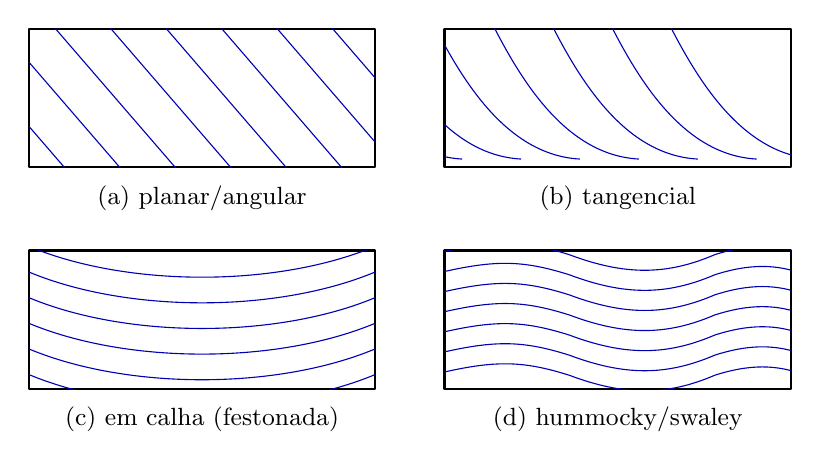
\begin{tikzpicture}[line cap=round,line join=round,scale=0.88,
                    every node/.style={font=\small}]
  % (a) Planar/angular: limites planos e lâminas inclinadas retas.
  \begin{scope}[shift={(0,3.2)}]
    \draw[thick] (0,0) rectangle (5,2);
    \begin{scope}
      \clip (0,0) rectangle (5,2);
      \foreach \x in {-1.3,-0.5,0.3,1.1,1.9,2.7,3.5,4.3} {
        \draw[blue!70!black] (\x,2.1)--({\x+1.9},-0.1);
      }
    \end{scope}
    \node[below] at (2.5,-0.12) {(a) planar/angular};
  \end{scope}
  % (b) Tangencial: lâminas se achatam ao aproximar-se da base.
  \begin{scope}[shift={(6,3.2)}]
    \draw[thick] (0,0) rectangle (5,2);
    \begin{scope}
      \clip (0,0) rectangle (5,2);
      \foreach \x in {-1.9,-1.05,-0.2,0.65,1.5,2.35,3.2} {
        \draw[blue!70!black] (\x,2.15)
          .. controls ({\x+0.45},1.25) and ({\x+1.1},0.18) ..
          ({\x+2.15},0.12);
      }
    \end{scope}
    \node[below] at (2.5,-0.12) {(b) tangencial};
  \end{scope}
  % (c) Calha: cortes côncavos sucessivos.
  \begin{scope}[shift={(0,0)}]
    \draw[thick] (0,0) rectangle (5,2);
    \begin{scope}
      \clip (0,0) rectangle (5,2);
      \foreach \h in {0.35,0.72,1.09,1.46,1.83,2.20} {
        \draw[blue!70!black] (-0.3,\h)
          .. controls (1.2,{\h-0.78}) and (3.8,{\h-0.78}) ..
          (5.3,\h);
      }
    \end{scope}
    \node[below] at (2.5,-0.12) {(c) em calha (festonada)};
  \end{scope}
  % (d) Hummocky/swaley: laminações onduladas de baixo ângulo.
  \begin{scope}[shift={(6,0)}]
    \draw[thick] (0,0) rectangle (5,2);
    \begin{scope}
      \clip (0,0) rectangle (5,2);
      \foreach \h in {0.20,0.49,0.78,1.07,1.36,1.65,1.94} {
        \draw[blue!70!black] (-0.2,\h)
          .. controls (0.7,{\h+0.22}) and (1.1,{\h+0.22}) ..
          (1.8,\h)
          .. controls (2.6,{\h-0.30}) and (3.2,{\h-0.30}) ..
          (3.9,\h)
          .. controls (4.4,{\h+0.16}) and (4.8,{\h+0.16}) ..
          (5.2,\h);
      }
    \end{scope}
    \node[below] at (2.5,-0.12) {(d) hummocky/swaley};
  \end{scope}
\end{tikzpicture}
\caption{Comparação esquemática de geometrias internas de estratificação.
Os retângulos representam os limites externos de cada intervalo; as linhas
azuis representam lâminas preservadas. O quadro (d) representa estruturas
de ondas e fluxos combinados, não a migração simples de uma duna.
Desenhos sem escala.}
\label{fig:tipos-estratificacao}
\end{figure}

\subsection{Seixos imbricados}

\emph{Imbricação} é o arranjo preferencial de clastos, sobretudo seixos
achatados, que se sobrepõem como telhas. Em muitos depósitos de corrente,
seus planos mergulham para montante. A orientação de vários seixos pode
indicar a paleocorrente, mas uma pedra isolada não é suficiente; deve-se
verificar também se a camada não foi inclinada posteriormente.

\begin{figure}[htbp]
\centering
\begin{tikzpicture}[>=Stealth,scale=0.83]
  \draw[->,thick] (3.3,1.5)--(5.4,1.5) node[right]{fluxo};
  \draw[thick] (0,0)--(6.3,0);
  \foreach \x in {0.8,1.7,2.6,3.5,4.4,5.3} {
    \draw[thick,rotate around={25:(\x,0.52)}]
      (\x,0.52) ellipse (0.62 and 0.19);
  }
  \node[below] at (1,-0.1) {montante};
  \node[below] at (5.1,-0.1) {jusante};
\end{tikzpicture}
\caption{Seixos imbricados com planos mergulhando para montante.
Esquema sem escala.}
\label{fig:seixos-imbricados}
\end{figure}

\subsection{Forma dos grãos e feições superficiais}

A forma de um grão inclui sua esfericidade, seu arredondamento e, no caso
de clastos maiores, a proporção entre seus eixos. Suas feições superficiais
podem registrar episódios sucessivos de transporte, alteração e deformação.
Nenhuma marca isolada prova um ambiente de formação.

\begin{description}[leftmargin=2.7cm,style=nextline]
  \item[Facetas] Superfícies relativamente planas produzidas por desgaste,
  fratura ou contato com outros materiais. Devem ser interpretadas junto
  com outras feições e com o contexto do depósito.
  \item[Cavidades] Depressões ou marcas superficiais que podem decorrer de
  impactos, dissolução ou alteração. É preciso registrar tamanho, forma e
  distribuição antes de atribuir-lhes uma origem.
  \item[Achatamento] Forma em que uma dimensão do clasto é menor que as
  demais. Pode ser herdada da rocha fonte, resultar de desgaste seletivo ou
  de deformação posterior. Favorece a formação de arranjos imbricados.
  \item[Estrias] Riscos e sulcos estreitos produzidos por abrasão ou atrito.
  Podem ocorrer em clastos transportados por geleiras, mas uma interpretação
  glacial requer outras evidências associadas
  \autocite{trosdtorf2005glacial}.
\end{description}

\subsection{Camadas maciças e deformação de sedimentos moles}

Uma camada \emph{maciça} não apresenta laminação interna facilmente
reconhecível na escala observada. Trata-se de uma descrição, não de um
processo único. A aparência pode resultar de sedimentação rápida de
material relativamente homogêneo, deposição por fluxos concentrados,
mistura biológica que apagou estruturas anteriores ou ausência de
contrastes visíveis entre lâminas \autocite{iodpestrutura,iodpbioturbacao}.

Fluxos de detritos ricos em sedimentos podem comportar-se como misturas
viscosas, transportando partículas de tamanhos diversos. Para interpretar
uma camada como produto desse processo, observam-se também seleção,
suporte dos clastos, contatos e associação com outras fácies. A aparência
maciça, sozinha, não é diagnóstica.

\paragraph{Escape de fluido.}
Sedimentos recém-depositados podem conservar muita água nos poros.
Sob carregamento rápido, a água escapa e pode deformar as laminações,
formar condutos ou produzir pequenos vulcões de areia. Essas feições
indicam mobilização após a deposição inicial e antes da completa
consolidação \autocite{kgsheterolitica}.

\paragraph{Dobramento sedimentar.}
Um escorregamento de sedimentos ainda pouco consolidados pode inclinar
e dobrar camadas; laminações convolutas também podem ocorrer em intervalos
restritos. Para distinguir esse dobramento de deformação tectônica
posterior, examinam-se os limites do intervalo deformado, as camadas
vizinhas e sua relação com o relevo deposicional
\autocite{kgsheterolitica}.

\subsection{Bioturbação, traços fósseis e icnofósseis}

\emph{Bioturbação} é a perturbação do sedimento pela atividade de
organismos, incluindo escavação, alimentação e deslocamento. Ela pode
preservar galerias reconhecíveis ou destruir quase toda a laminação,
deixando uma textura aparentemente homogênea \autocite{iodpbioturbacao}.

\emph{Traço fóssil} e \emph{icnofóssil} são nomes equivalentes para a
evidência preservada de atividade biológica, como pistas e galerias.
Bioturbação nomeia o processo e seu efeito sobre o sedimento; nem toda
camada bioturbada conserva um traço individual identificável
\autocite{kuichnologia}.

\subsection{Gretas de ressecamento e argilominerais}

\emph{Gretas de ressecamento} se abrem quando um sedimento úmido perde
água e se contrai. Em planta, podem delimitar polígonos; em corte,
frequentemente se estreitam para baixo. O preenchimento posterior
das fendas pode preservar seu molde nas rochas. Elas indicam exposição
e perda de água, embora seja necessário distinguir outras causas de
fraturamento por meio do contexto sedimentar.

Os argilominerais pertencem aos \emph{filossilicatos}, minerais de
estrutura em folhas. Alguns, especialmente os do grupo da esmectita,
incorporam água entre camadas e podem expandir-se ao hidratar e contrair
ao secar. Essa variação pode favorecer o desenvolvimento de gretas.
Nem todos os argilominerais são igualmente expansivos; a greta, sozinha,
não identifica sua composição \autocite{usgsargilas}.

\subsection{Estruturas heterolíticas}

Depósitos \emph{heterolíticos} alternam areia e lama. Correntes mais
ativas podem transportar areia junto ao fundo, ao passo que a lama se
acumula durante intervalos de menor energia. Essa alternância ocorre
frequentemente em ambientes influenciados por marés, mas não é exclusiva
deles \autocite{kgsheterolitica}.

\begin{description}[leftmargin=3.1cm,style=nextline]
  \item[Acamamento flaser] Predomina a areia; finas porções descontínuas
  de lama podem ocupar as depressões de ripples arenosos.
  \item[Acamamento ondulado] Areia e lama formam lâminas onduladas mais
  contínuas, com presença relativamente equilibrada dos dois materiais.
  \item[Acamamento lenticular] Predomina a lama, com lentes de areia
  isoladas ou pouco conectadas.
\end{description}

Para sustentar uma interpretação de marés, convém procurar também
reversão de paleocorrentes, superfícies de reativação e outras evidências
na associação de fácies \autocite{kgsheterolitica}.

\subsection{Marcas de sola, turboglifos e marcas de objeto}

\emph{Marcas de sola} são feições preservadas na superfície inferior de
uma camada. Muitas começam como depressões escavadas em lama; a areia
depositada depois as preenche e conserva um contramolde em relevo na
base do arenito \autocite{solemarks1957}.

\paragraph{Turboglifos.}
Os turboglifos (\emph{flute marks}) são escavações alongadas e assimétricas
produzidas pelo fluxo sobre um fundo coeso. Seus contramoldes são os
\emph{flute casts}. No caso típico, a extremidade mais larga e abrupta
aponta para montante e a parte afilada se prolonga para jusante,
indicando o sentido da paleocorrente \autocite{solemarks1957,kgssolemarks}.

\paragraph{Marcas de objeto.}
Seixos, conchas e fragmentos transportados podem tocar, arrastar-se ou
ricochetear no fundo, produzindo sulcos e marcas de impacto
(\emph{tool marks}). Sulcos longos frequentemente indicam a orientação
do movimento, mas nem sempre seu sentido. Turboglifos e marcas de objeto
são tipos distintos de marcas que podem ser preservadas na sola de uma
camada \autocite{solemarks1957}.

% ----------------------------------------------------------------------
% REFERÊNCIAS NOVAS: copie as entradas abaixo, SEM o sinal % inicial,
% para o arquivo referencias.bib que já acompanha seu documento.
% A entrada trosdtorf2005glacial foi fornecida anteriormente.
%
% @online{southard2006bedforms,
%   author = {Southard, John},
%   title = {Bed Configurations Generated by Water Flows and Wind},
%   organization = {MIT OpenCourseWare}, year = {2006},
%   url = {https://ocw.mit.edu/courses/12-090-introduction-to-fluid-motions-sediment-transport-and-current-generated-sedimentary-structures-fall-2006/resources/ch12/},
%   urldate = {2026-09-28}}
% @online{southard2006cross,
%   author = {Southard, John}, title = {Cross Stratification},
%   organization = {MIT OpenCourseWare}, year = {2006},
%   url = {https://ocw.mit.edu/courses/12-090-introduction-to-fluid-motions-sediment-transport-and-current-generated-sedimentary-structures-fall-2006/resources/ch16/},
%   urldate = {2026-09-28}}
% @online{iodpestrutura,
%   author = {{International Ocean Discovery Program}},
%   title = {Sediment Description: Sedimentary Structures},
%   url = {https://iodp.tamu.edu/publications/TN/Appendix/Appendix_4.1.pdf},
%   urldate = {2026-09-28}}
% @online{iodpbioturbacao,
%   author = {{Ocean Drilling Program}}, title = {Methods: Sediment Description},
%   url = {https://www.iodp.tamu.edu/publications/exp302/103/103_2.htm},
%   urldate = {2026-09-28}}
% @online{kgsheterolitica,
%   author = {{Kansas Geological Survey}},
%   title = {Sedimentology and Ichnology of Paleozoic Estuarine and Shoreface Reservoirs},
%   url = {https://www.kgs.ku.edu/Current/1999/buatois/buatois5.html},
%   urldate = {2026-09-28}}
% @online{kuichnologia,
%   author = {{University of Kansas}}, title = {Glossary: Ichnology},
%   url = {https://ichnology.ku.edu/poi/poi/glossary.html},
%   urldate = {2026-09-28}}
% @online{usgsargilas,
%   author = {{U.S. Geological Survey}},
%   title = {Environmental Characteristics of Clays and Clay Mineral Deposits},
%   url = {https://pubs.usgs.gov/info/clays/},
%   urldate = {2026-09-28}}
% @article{solemarks1957,
%   title = {Sole Markings of Graded Graywacke Beds},
%   journaltitle = {The Journal of Geology}, year = {1957},
%   volume = {65}, number = {3}, doi = {10.1086/626429}}
% @online{kgssolemarks,
%   author = {{Kansas Geological Survey}},
%   title = {Ichnology of a Pennsylvanian Equatorial Tidal Flat: Sedimentology},
%   url = {https://www.kgs.ku.edu/Publications/Bulletins/245/03_sedim.html},
%   urldate = {2026-09-28}}
% @online{usgshummocky,
%   author = {{U.S. Geological Survey}},
%   title = {Cyclic Deposits and Hummocky Cross-Stratification of Probable
%            Storm Origins in Upper Cretaceous Rocks of the Cape Sebastian Area},
%   url = {https://pubs.usgs.gov/publication/70011848},
%   urldate = {2026-09-29}}
.
% Requer os pacotes tikz, graphicx, enumitem e biblatex já presentes no preâmbulo.
% As entradas bibliográficas correspondentes estão comentadas no fim deste arquivo.

\section{Formas de leito e estruturas sedimentares}

As formas de leito são irregularidades produzidas na superfície de sedimentos
soltos por correntes, ondas ou vento. Durante sua migração, uma parte do leito
é erodida e outra recebe novos grãos. Por isso, o relevo original nem sempre
se conserva: frequentemente permanecem as lâminas inclinadas depositadas
durante a migração. É importante distinguir a forma superficial, sua estrutura
interna preservada e a interpretação do fluxo que a produziu
\autocite{southard2006bedforms,southard2006cross}.

\subsection{Ripples e dunas}

\paragraph{Ripples de corrente.}
Ripples são ondulações pequenas do leito. Sob um fluxo predominantemente
unidirecional, costumam ser assimétricos: o flanco de montante é relativamente
suave e a face de jusante, mais íngreme. Os grãos avançam sobre a primeira
face e se acumulam na segunda. A migração sucessiva pode deixar
\emph{laminação cruzada} de pequena escala. A orientação das lâminas fornece
uma indicação de paleocorrente, desde que a posição original das camadas
tenha sido considerada \autocite{southard2006cross}.

\paragraph{Ripples de ondas.}
Sob movimentos oscilatórios da água, os dois flancos podem ter inclinações
semelhantes. Correntes combinadas com ondas, entretanto, também produzem
formas assimétricas. Assim, a simetria é uma pista, não uma prova isolada da
origem da estrutura \autocite{southard2006bedforms}.

\begin{figure}[htbp]
\centering
\begin{tikzpicture}[>=Stealth,scale=0.8]
  \draw[->,thick] (0,1.6)--(2,1.6) node[right]{corrente};
  \draw[thick] plot[smooth] coordinates {
    (0,0) (0.6,0.1) (1.5,0.42) (2.1,0.85) (2.45,0.2)
    (2.8,0) (3.4,0.1) (4.3,0.42) (4.9,0.85) (5.25,0.2) (5.6,0)};
  \draw[thin] (2.15,0.68)--(2.47,0.07);
  \draw[thin] (2.25,0.56)--(2.57,0.03);
  \draw[thin] (4.95,0.68)--(5.27,0.07);
  \draw[thin] (5.05,0.56)--(5.37,0.03);
  \node[below] at (1.25,-0.1) {flanco suave};
  \node[below] at (4.1,-0.1) {face de jusante};
\end{tikzpicture}
\caption{Ripples assimétricos de corrente e lâminas na face de jusante.
Esquema sem escala.}
\label{fig:ripples-corrente}
\end{figure}

\paragraph{Dunas.}
As dunas são formas de leito maiores que os ripples e ocorrem em ambientes
subaquosos e eólicos. Ao migrarem, depositam camadas inclinadas na face de
jusante. A erosão posterior pode remover a crista e parte do depósito,
preservando apenas conjuntos de \emph{estratificação cruzada}. A espessura
desse conjunto não equivale necessariamente à altura da duna original
\autocite{southard2006bedforms,southard2006cross}.

Uma \emph{superfície de reativação} corta lâminas já formadas e é recoberta
por novas lâminas. Registra uma mudança nas condições do fluxo e a retomada
da deposição; não exige, por si só, uma inversão da corrente. A
Figura~\ref{fig:duna-reativacao} representa essa relação.

\begin{figure}[htbp]
\centering
\begin{tikzpicture}[>=Stealth,scale=0.86,
                    every node/.style={font=\small}]
  \draw[very thick] (0.5,0.6)--(10.5,0.6);
  \draw[very thick]
    (0.5,3.15) .. controls (2,3.25) and (3.1,3.65) .. (4,3.75)
    .. controls (5.3,3.35) and (6.1,2.55) .. (7,2.10)
    .. controls (8,1.65) and (9.2,1.55) .. (10.5,1.70);
  \begin{scope}
    \clip (0.5,0.6)--(10.5,0.6)--(8.5,1.32)
      .. controls (7,1.52) and (5.3,2.10) .. (4.35,2.63)
      --(0.5,3.15)--cycle;
    \foreach \s in {0,0.55,1.10,1.65,2.20,2.75,3.30} {
      \draw[blue!70!black,thick] ({1.35+\s},3.65)
        .. controls ({3+\s},3.05) and ({4.2+\s},1.2) ..
        ({5.25+\s},0.6);
    }
  \end{scope}
  \begin{scope}
    \clip (4.35,2.63) .. controls (5.3,2.10) and (7,1.52) ..
      (8.5,1.32)--(10.5,1.7)--(10.5,4.1)--(4,4.1)--cycle;
    \foreach \s in {0,0.50,1.00,1.50,2.00} {
      \draw[orange!85!black,thick] ({4.20+\s},3.75)
        .. controls ({5+\s},3.25) and ({5.8+\s},2.05) ..
        ({6.65+\s},1.25);
    }
  \end{scope}
  \draw[red!75!black,very thick] (4.35,2.63)
    .. controls (5.3,2.10) and (7,1.52) .. (8.5,1.32);
  \draw[->,thick] (0.75,4.45)--(2.55,4.45)
    node[right]{migração da duna};
  \node[blue!70!black] at (2.3,1.4) {lâminas antigas};
  \node[orange!85!black,align=center] at (8.8,3.0)
    {lâminas novas};
  \node[red!75!black,align=center] at (9.5,3.8)
    {superfície de\\reativação};
  \draw[->,red!75!black,thick] (9.3,3.3)--(7.5,1.62);
  \node[below] at (5.5,0.55) {superfície basal};
\end{tikzpicture}
\caption{Duna com estratificação cruzada: a superfície de reativação
trunca lâminas antigas e é recoberta por lâminas novas. Esquema sem escala.}
\label{fig:duna-reativacao}
\end{figure}

\paragraph{Geometria das lâminas preservadas.}
A Figura~\ref{fig:tipos-estratificacao} compara quatro geometrias internas.
Nos dois primeiros quadros, as lâminas inclinadas são aproximadamente
retas ou tornam-se tangentes à base do conjunto. Em uma calha, a geometria
é tridimensional: um corte vertical mostra lâminas côncavas, mas a aparência
varia com a orientação do corte. A estratificação \emph{hummocky/swaley}
apresenta ondulações suaves, com altos e baixos de baixo ângulo, geralmente
associadas à ação combinada de ondas e correntes durante tempestades.
Ela foi incluída para comparar padrões internos, mas não deve ser
interpretada automaticamente como depósito de uma duna migrante
\autocite{southard2006cross,usgshummocky}.

\begin{figure}[htbp]
\centering
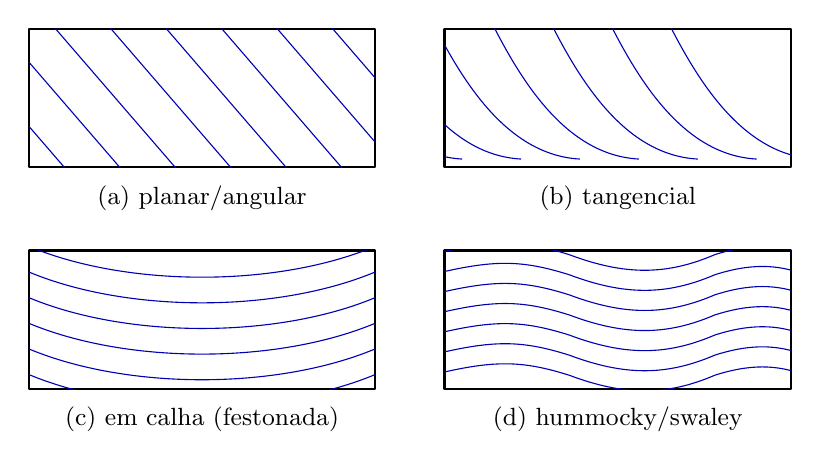
\begin{tikzpicture}[line cap=round,line join=round,scale=0.88,
                    every node/.style={font=\small}]
  % (a) Planar/angular: limites planos e lâminas inclinadas retas.
  \begin{scope}[shift={(0,3.2)}]
    \draw[thick] (0,0) rectangle (5,2);
    \begin{scope}
      \clip (0,0) rectangle (5,2);
      \foreach \x in {-1.3,-0.5,0.3,1.1,1.9,2.7,3.5,4.3} {
        \draw[blue!70!black] (\x,2.1)--({\x+1.9},-0.1);
      }
    \end{scope}
    \node[below] at (2.5,-0.12) {(a) planar/angular};
  \end{scope}
  % (b) Tangencial: lâminas se achatam ao aproximar-se da base.
  \begin{scope}[shift={(6,3.2)}]
    \draw[thick] (0,0) rectangle (5,2);
    \begin{scope}
      \clip (0,0) rectangle (5,2);
      \foreach \x in {-1.9,-1.05,-0.2,0.65,1.5,2.35,3.2} {
        \draw[blue!70!black] (\x,2.15)
          .. controls ({\x+0.45},1.25) and ({\x+1.1},0.18) ..
          ({\x+2.15},0.12);
      }
    \end{scope}
    \node[below] at (2.5,-0.12) {(b) tangencial};
  \end{scope}
  % (c) Calha: cortes côncavos sucessivos.
  \begin{scope}[shift={(0,0)}]
    \draw[thick] (0,0) rectangle (5,2);
    \begin{scope}
      \clip (0,0) rectangle (5,2);
      \foreach \h in {0.35,0.72,1.09,1.46,1.83,2.20} {
        \draw[blue!70!black] (-0.3,\h)
          .. controls (1.2,{\h-0.78}) and (3.8,{\h-0.78}) ..
          (5.3,\h);
      }
    \end{scope}
    \node[below] at (2.5,-0.12) {(c) em calha (festonada)};
  \end{scope}
  % (d) Hummocky/swaley: laminações onduladas de baixo ângulo.
  \begin{scope}[shift={(6,0)}]
    \draw[thick] (0,0) rectangle (5,2);
    \begin{scope}
      \clip (0,0) rectangle (5,2);
      \foreach \h in {0.20,0.49,0.78,1.07,1.36,1.65,1.94} {
        \draw[blue!70!black] (-0.2,\h)
          .. controls (0.7,{\h+0.22}) and (1.1,{\h+0.22}) ..
          (1.8,\h)
          .. controls (2.6,{\h-0.30}) and (3.2,{\h-0.30}) ..
          (3.9,\h)
          .. controls (4.4,{\h+0.16}) and (4.8,{\h+0.16}) ..
          (5.2,\h);
      }
    \end{scope}
    \node[below] at (2.5,-0.12) {(d) hummocky/swaley};
  \end{scope}
\end{tikzpicture}
\caption{Comparação esquemática de geometrias internas de estratificação.
Os retângulos representam os limites externos de cada intervalo; as linhas
azuis representam lâminas preservadas. O quadro (d) representa estruturas
de ondas e fluxos combinados, não a migração simples de uma duna.
Desenhos sem escala.}
\label{fig:tipos-estratificacao}
\end{figure}

\subsection{Seixos imbricados}

\emph{Imbricação} é o arranjo preferencial de clastos, sobretudo seixos
achatados, que se sobrepõem como telhas. Em muitos depósitos de corrente,
seus planos mergulham para montante. A orientação de vários seixos pode
indicar a paleocorrente, mas uma pedra isolada não é suficiente; deve-se
verificar também se a camada não foi inclinada posteriormente.

\begin{figure}[htbp]
\centering
\begin{tikzpicture}[>=Stealth,scale=0.83]
  \draw[->,thick] (3.3,1.5)--(5.4,1.5) node[right]{fluxo};
  \draw[thick] (0,0)--(6.3,0);
  \foreach \x in {0.8,1.7,2.6,3.5,4.4,5.3} {
    \draw[thick,rotate around={25:(\x,0.52)}]
      (\x,0.52) ellipse (0.62 and 0.19);
  }
  \node[below] at (1,-0.1) {montante};
  \node[below] at (5.1,-0.1) {jusante};
\end{tikzpicture}
\caption{Seixos imbricados com planos mergulhando para montante.
Esquema sem escala.}
\label{fig:seixos-imbricados}
\end{figure}

\subsection{Forma dos grãos e feições superficiais}

A forma de um grão inclui sua esfericidade, seu arredondamento e, no caso
de clastos maiores, a proporção entre seus eixos. Suas feições superficiais
podem registrar episódios sucessivos de transporte, alteração e deformação.
Nenhuma marca isolada prova um ambiente de formação.

\begin{description}[leftmargin=2.7cm,style=nextline]
  \item[Facetas] Superfícies relativamente planas produzidas por desgaste,
  fratura ou contato com outros materiais. Devem ser interpretadas junto
  com outras feições e com o contexto do depósito.
  \item[Cavidades] Depressões ou marcas superficiais que podem decorrer de
  impactos, dissolução ou alteração. É preciso registrar tamanho, forma e
  distribuição antes de atribuir-lhes uma origem.
  \item[Achatamento] Forma em que uma dimensão do clasto é menor que as
  demais. Pode ser herdada da rocha fonte, resultar de desgaste seletivo ou
  de deformação posterior. Favorece a formação de arranjos imbricados.
  \item[Estrias] Riscos e sulcos estreitos produzidos por abrasão ou atrito.
  Podem ocorrer em clastos transportados por geleiras, mas uma interpretação
  glacial requer outras evidências associadas
  \autocite{trosdtorf2005glacial}.
\end{description}

\subsection{Camadas maciças e deformação de sedimentos moles}

Uma camada \emph{maciça} não apresenta laminação interna facilmente
reconhecível na escala observada. Trata-se de uma descrição, não de um
processo único. A aparência pode resultar de sedimentação rápida de
material relativamente homogêneo, deposição por fluxos concentrados,
mistura biológica que apagou estruturas anteriores ou ausência de
contrastes visíveis entre lâminas \autocite{iodpestrutura,iodpbioturbacao}.

Fluxos de detritos ricos em sedimentos podem comportar-se como misturas
viscosas, transportando partículas de tamanhos diversos. Para interpretar
uma camada como produto desse processo, observam-se também seleção,
suporte dos clastos, contatos e associação com outras fácies. A aparência
maciça, sozinha, não é diagnóstica.

\paragraph{Escape de fluido.}
Sedimentos recém-depositados podem conservar muita água nos poros.
Sob carregamento rápido, a água escapa e pode deformar as laminações,
formar condutos ou produzir pequenos vulcões de areia. Essas feições
indicam mobilização após a deposição inicial e antes da completa
consolidação \autocite{kgsheterolitica}.

\paragraph{Dobramento sedimentar.}
Um escorregamento de sedimentos ainda pouco consolidados pode inclinar
e dobrar camadas; laminações convolutas também podem ocorrer em intervalos
restritos. Para distinguir esse dobramento de deformação tectônica
posterior, examinam-se os limites do intervalo deformado, as camadas
vizinhas e sua relação com o relevo deposicional
\autocite{kgsheterolitica}.

\subsection{Bioturbação, traços fósseis e icnofósseis}

\emph{Bioturbação} é a perturbação do sedimento pela atividade de
organismos, incluindo escavação, alimentação e deslocamento. Ela pode
preservar galerias reconhecíveis ou destruir quase toda a laminação,
deixando uma textura aparentemente homogênea \autocite{iodpbioturbacao}.

\emph{Traço fóssil} e \emph{icnofóssil} são nomes equivalentes para a
evidência preservada de atividade biológica, como pistas e galerias.
Bioturbação nomeia o processo e seu efeito sobre o sedimento; nem toda
camada bioturbada conserva um traço individual identificável
\autocite{kuichnologia}.

\subsection{Gretas de ressecamento e argilominerais}

\emph{Gretas de ressecamento} se abrem quando um sedimento úmido perde
água e se contrai. Em planta, podem delimitar polígonos; em corte,
frequentemente se estreitam para baixo. O preenchimento posterior
das fendas pode preservar seu molde nas rochas. Elas indicam exposição
e perda de água, embora seja necessário distinguir outras causas de
fraturamento por meio do contexto sedimentar.

Os argilominerais pertencem aos \emph{filossilicatos}, minerais de
estrutura em folhas. Alguns, especialmente os do grupo da esmectita,
incorporam água entre camadas e podem expandir-se ao hidratar e contrair
ao secar. Essa variação pode favorecer o desenvolvimento de gretas.
Nem todos os argilominerais são igualmente expansivos; a greta, sozinha,
não identifica sua composição \autocite{usgsargilas}.

\subsection{Estruturas heterolíticas}

Depósitos \emph{heterolíticos} alternam areia e lama. Correntes mais
ativas podem transportar areia junto ao fundo, ao passo que a lama se
acumula durante intervalos de menor energia. Essa alternância ocorre
frequentemente em ambientes influenciados por marés, mas não é exclusiva
deles \autocite{kgsheterolitica}.

\begin{description}[leftmargin=3.1cm,style=nextline]
  \item[Acamamento flaser] Predomina a areia; finas porções descontínuas
  de lama podem ocupar as depressões de ripples arenosos.
  \item[Acamamento ondulado] Areia e lama formam lâminas onduladas mais
  contínuas, com presença relativamente equilibrada dos dois materiais.
  \item[Acamamento lenticular] Predomina a lama, com lentes de areia
  isoladas ou pouco conectadas.
\end{description}

Para sustentar uma interpretação de marés, convém procurar também
reversão de paleocorrentes, superfícies de reativação e outras evidências
na associação de fácies \autocite{kgsheterolitica}.

\subsection{Marcas de sola, turboglifos e marcas de objeto}

\emph{Marcas de sola} são feições preservadas na superfície inferior de
uma camada. Muitas começam como depressões escavadas em lama; a areia
depositada depois as preenche e conserva um contramolde em relevo na
base do arenito \autocite{solemarks1957}.

\paragraph{Turboglifos.}
Os turboglifos (\emph{flute marks}) são escavações alongadas e assimétricas
produzidas pelo fluxo sobre um fundo coeso. Seus contramoldes são os
\emph{flute casts}. No caso típico, a extremidade mais larga e abrupta
aponta para montante e a parte afilada se prolonga para jusante,
indicando o sentido da paleocorrente \autocite{solemarks1957,kgssolemarks}.

\paragraph{Marcas de objeto.}
Seixos, conchas e fragmentos transportados podem tocar, arrastar-se ou
ricochetear no fundo, produzindo sulcos e marcas de impacto
(\emph{tool marks}). Sulcos longos frequentemente indicam a orientação
do movimento, mas nem sempre seu sentido. Turboglifos e marcas de objeto
são tipos distintos de marcas que podem ser preservadas na sola de uma
camada \autocite{solemarks1957}.

% ----------------------------------------------------------------------
% REFERÊNCIAS NOVAS: copie as entradas abaixo, SEM o sinal % inicial,
% para o arquivo referencias.bib que já acompanha seu documento.
% A entrada trosdtorf2005glacial foi fornecida anteriormente.
%
% @online{southard2006bedforms,
%   author = {Southard, John},
%   title = {Bed Configurations Generated by Water Flows and Wind},
%   organization = {MIT OpenCourseWare}, year = {2006},
%   url = {https://ocw.mit.edu/courses/12-090-introduction-to-fluid-motions-sediment-transport-and-current-generated-sedimentary-structures-fall-2006/resources/ch12/},
%   urldate = {2026-09-28}}
% @online{southard2006cross,
%   author = {Southard, John}, title = {Cross Stratification},
%   organization = {MIT OpenCourseWare}, year = {2006},
%   url = {https://ocw.mit.edu/courses/12-090-introduction-to-fluid-motions-sediment-transport-and-current-generated-sedimentary-structures-fall-2006/resources/ch16/},
%   urldate = {2026-09-28}}
% @online{iodpestrutura,
%   author = {{International Ocean Discovery Program}},
%   title = {Sediment Description: Sedimentary Structures},
%   url = {https://iodp.tamu.edu/publications/TN/Appendix/Appendix_4.1.pdf},
%   urldate = {2026-09-28}}
% @online{iodpbioturbacao,
%   author = {{Ocean Drilling Program}}, title = {Methods: Sediment Description},
%   url = {https://www.iodp.tamu.edu/publications/exp302/103/103_2.htm},
%   urldate = {2026-09-28}}
% @online{kgsheterolitica,
%   author = {{Kansas Geological Survey}},
%   title = {Sedimentology and Ichnology of Paleozoic Estuarine and Shoreface Reservoirs},
%   url = {https://www.kgs.ku.edu/Current/1999/buatois/buatois5.html},
%   urldate = {2026-09-28}}
% @online{kuichnologia,
%   author = {{University of Kansas}}, title = {Glossary: Ichnology},
%   url = {https://ichnology.ku.edu/poi/poi/glossary.html},
%   urldate = {2026-09-28}}
% @online{usgsargilas,
%   author = {{U.S. Geological Survey}},
%   title = {Environmental Characteristics of Clays and Clay Mineral Deposits},
%   url = {https://pubs.usgs.gov/info/clays/},
%   urldate = {2026-09-28}}
% @article{solemarks1957,
%   title = {Sole Markings of Graded Graywacke Beds},
%   journaltitle = {The Journal of Geology}, year = {1957},
%   volume = {65}, number = {3}, doi = {10.1086/626429}}
% @online{kgssolemarks,
%   author = {{Kansas Geological Survey}},
%   title = {Ichnology of a Pennsylvanian Equatorial Tidal Flat: Sedimentology},
%   url = {https://www.kgs.ku.edu/Publications/Bulletins/245/03_sedim.html},
%   urldate = {2026-09-28}}
% @online{usgshummocky,
%   author = {{U.S. Geological Survey}},
%   title = {Cyclic Deposits and Hummocky Cross-Stratification of Probable
%            Storm Origins in Upper Cretaceous Rocks of the Cape Sebastian Area},
%   url = {https://pubs.usgs.gov/publication/70011848},
%   urldate = {2026-09-29}}
.
% Requer os pacotes tikz, graphicx, enumitem e biblatex já presentes no preâmbulo.
% As entradas bibliográficas correspondentes estão comentadas no fim deste arquivo.

\section{Formas de leito e estruturas sedimentares}

As formas de leito são irregularidades produzidas na superfície de sedimentos
soltos por correntes, ondas ou vento. Durante sua migração, uma parte do leito
é erodida e outra recebe novos grãos. Por isso, o relevo original nem sempre
se conserva: frequentemente permanecem as lâminas inclinadas depositadas
durante a migração. É importante distinguir a forma superficial, sua estrutura
interna preservada e a interpretação do fluxo que a produziu
\autocite{southard2006bedforms,southard2006cross}.

\subsection{Ripples e dunas}

\paragraph{Ripples de corrente.}
Ripples são ondulações pequenas do leito. Sob um fluxo predominantemente
unidirecional, costumam ser assimétricos: o flanco de montante é relativamente
suave e a face de jusante, mais íngreme. Os grãos avançam sobre a primeira
face e se acumulam na segunda. A migração sucessiva pode deixar
\emph{laminação cruzada} de pequena escala. A orientação das lâminas fornece
uma indicação de paleocorrente, desde que a posição original das camadas
tenha sido considerada \autocite{southard2006cross}.

\paragraph{Ripples de ondas.}
Sob movimentos oscilatórios da água, os dois flancos podem ter inclinações
semelhantes. Correntes combinadas com ondas, entretanto, também produzem
formas assimétricas. Assim, a simetria é uma pista, não uma prova isolada da
origem da estrutura \autocite{southard2006bedforms}.

\begin{figure}[htbp]
\centering
\begin{tikzpicture}[>=Stealth,scale=0.8]
  \draw[->,thick] (0,1.6)--(2,1.6) node[right]{corrente};
  \draw[thick] plot[smooth] coordinates {
    (0,0) (0.6,0.1) (1.5,0.42) (2.1,0.85) (2.45,0.2)
    (2.8,0) (3.4,0.1) (4.3,0.42) (4.9,0.85) (5.25,0.2) (5.6,0)};
  \draw[thin] (2.15,0.68)--(2.47,0.07);
  \draw[thin] (2.25,0.56)--(2.57,0.03);
  \draw[thin] (4.95,0.68)--(5.27,0.07);
  \draw[thin] (5.05,0.56)--(5.37,0.03);
  \node[below] at (1.25,-0.1) {flanco suave};
  \node[below] at (4.1,-0.1) {face de jusante};
\end{tikzpicture}
\caption{Ripples assimétricos de corrente e lâminas na face de jusante.
Esquema sem escala.}
\label{fig:ripples-corrente}
\end{figure}

\paragraph{Dunas.}
As dunas são formas de leito maiores que os ripples e ocorrem em ambientes
subaquosos e eólicos. Ao migrarem, depositam camadas inclinadas na face de
jusante. A erosão posterior pode remover a crista e parte do depósito,
preservando apenas conjuntos de \emph{estratificação cruzada}. A espessura
desse conjunto não equivale necessariamente à altura da duna original
\autocite{southard2006bedforms,southard2006cross}.

Uma \emph{superfície de reativação} corta lâminas já formadas e é recoberta
por novas lâminas. Registra uma mudança nas condições do fluxo e a retomada
da deposição; não exige, por si só, uma inversão da corrente. A
Figura~\ref{fig:duna-reativacao} representa essa relação.

\begin{figure}[htbp]
\centering
\begin{tikzpicture}[>=Stealth,scale=0.86,
                    every node/.style={font=\small}]
  \draw[very thick] (0.5,0.6)--(10.5,0.6);
  \draw[very thick]
    (0.5,3.15) .. controls (2,3.25) and (3.1,3.65) .. (4,3.75)
    .. controls (5.3,3.35) and (6.1,2.55) .. (7,2.10)
    .. controls (8,1.65) and (9.2,1.55) .. (10.5,1.70);
  \begin{scope}
    \clip (0.5,0.6)--(10.5,0.6)--(8.5,1.32)
      .. controls (7,1.52) and (5.3,2.10) .. (4.35,2.63)
      --(0.5,3.15)--cycle;
    \foreach \s in {0,0.55,1.10,1.65,2.20,2.75,3.30} {
      \draw[blue!70!black,thick] ({1.35+\s},3.65)
        .. controls ({3+\s},3.05) and ({4.2+\s},1.2) ..
        ({5.25+\s},0.6);
    }
  \end{scope}
  \begin{scope}
    \clip (4.35,2.63) .. controls (5.3,2.10) and (7,1.52) ..
      (8.5,1.32)--(10.5,1.7)--(10.5,4.1)--(4,4.1)--cycle;
    \foreach \s in {0,0.50,1.00,1.50,2.00} {
      \draw[orange!85!black,thick] ({4.20+\s},3.75)
        .. controls ({5+\s},3.25) and ({5.8+\s},2.05) ..
        ({6.65+\s},1.25);
    }
  \end{scope}
  \draw[red!75!black,very thick] (4.35,2.63)
    .. controls (5.3,2.10) and (7,1.52) .. (8.5,1.32);
  \draw[->,thick] (0.75,4.45)--(2.55,4.45)
    node[right]{migração da duna};
  \node[blue!70!black] at (2.3,1.4) {lâminas antigas};
  \node[orange!85!black,align=center] at (8.8,3.0)
    {lâminas novas};
  \node[red!75!black,align=center] at (9.5,3.8)
    {superfície de\\reativação};
  \draw[->,red!75!black,thick] (9.3,3.3)--(7.5,1.62);
  \node[below] at (5.5,0.55) {superfície basal};
\end{tikzpicture}
\caption{Duna com estratificação cruzada: a superfície de reativação
trunca lâminas antigas e é recoberta por lâminas novas. Esquema sem escala.}
\label{fig:duna-reativacao}
\end{figure}

\paragraph{Geometria das lâminas preservadas.}
A Figura~\ref{fig:tipos-estratificacao} compara quatro geometrias internas.
Nos dois primeiros quadros, as lâminas inclinadas são aproximadamente
retas ou tornam-se tangentes à base do conjunto. Em uma calha, a geometria
é tridimensional: um corte vertical mostra lâminas côncavas, mas a aparência
varia com a orientação do corte. A estratificação \emph{hummocky/swaley}
apresenta ondulações suaves, com altos e baixos de baixo ângulo, geralmente
associadas à ação combinada de ondas e correntes durante tempestades.
Ela foi incluída para comparar padrões internos, mas não deve ser
interpretada automaticamente como depósito de uma duna migrante
\autocite{southard2006cross,usgshummocky}.

\begin{figure}[htbp]
\centering
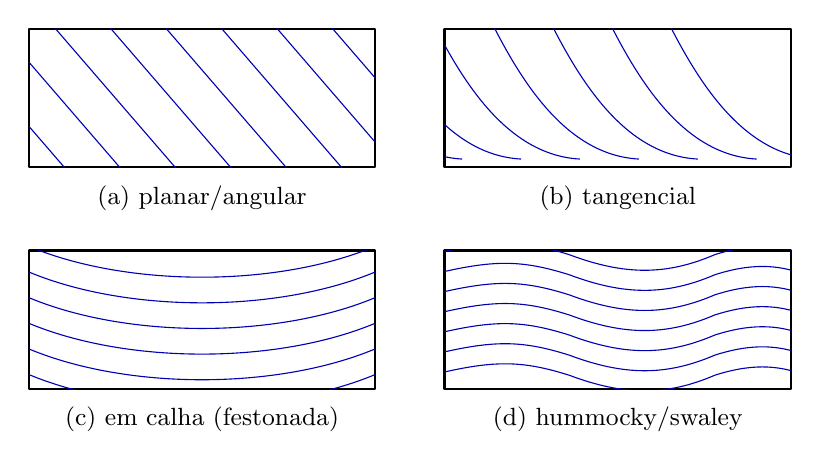
\begin{tikzpicture}[line cap=round,line join=round,scale=0.88,
                    every node/.style={font=\small}]
  % (a) Planar/angular: limites planos e lâminas inclinadas retas.
  \begin{scope}[shift={(0,3.2)}]
    \draw[thick] (0,0) rectangle (5,2);
    \begin{scope}
      \clip (0,0) rectangle (5,2);
      \foreach \x in {-1.3,-0.5,0.3,1.1,1.9,2.7,3.5,4.3} {
        \draw[blue!70!black] (\x,2.1)--({\x+1.9},-0.1);
      }
    \end{scope}
    \node[below] at (2.5,-0.12) {(a) planar/angular};
  \end{scope}
  % (b) Tangencial: lâminas se achatam ao aproximar-se da base.
  \begin{scope}[shift={(6,3.2)}]
    \draw[thick] (0,0) rectangle (5,2);
    \begin{scope}
      \clip (0,0) rectangle (5,2);
      \foreach \x in {-1.9,-1.05,-0.2,0.65,1.5,2.35,3.2} {
        \draw[blue!70!black] (\x,2.15)
          .. controls ({\x+0.45},1.25) and ({\x+1.1},0.18) ..
          ({\x+2.15},0.12);
      }
    \end{scope}
    \node[below] at (2.5,-0.12) {(b) tangencial};
  \end{scope}
  % (c) Calha: cortes côncavos sucessivos.
  \begin{scope}[shift={(0,0)}]
    \draw[thick] (0,0) rectangle (5,2);
    \begin{scope}
      \clip (0,0) rectangle (5,2);
      \foreach \h in {0.35,0.72,1.09,1.46,1.83,2.20} {
        \draw[blue!70!black] (-0.3,\h)
          .. controls (1.2,{\h-0.78}) and (3.8,{\h-0.78}) ..
          (5.3,\h);
      }
    \end{scope}
    \node[below] at (2.5,-0.12) {(c) em calha (festonada)};
  \end{scope}
  % (d) Hummocky/swaley: laminações onduladas de baixo ângulo.
  \begin{scope}[shift={(6,0)}]
    \draw[thick] (0,0) rectangle (5,2);
    \begin{scope}
      \clip (0,0) rectangle (5,2);
      \foreach \h in {0.20,0.49,0.78,1.07,1.36,1.65,1.94} {
        \draw[blue!70!black] (-0.2,\h)
          .. controls (0.7,{\h+0.22}) and (1.1,{\h+0.22}) ..
          (1.8,\h)
          .. controls (2.6,{\h-0.30}) and (3.2,{\h-0.30}) ..
          (3.9,\h)
          .. controls (4.4,{\h+0.16}) and (4.8,{\h+0.16}) ..
          (5.2,\h);
      }
    \end{scope}
    \node[below] at (2.5,-0.12) {(d) hummocky/swaley};
  \end{scope}
\end{tikzpicture}
\caption{Comparação esquemática de geometrias internas de estratificação.
Os retângulos representam os limites externos de cada intervalo; as linhas
azuis representam lâminas preservadas. O quadro (d) representa estruturas
de ondas e fluxos combinados, não a migração simples de uma duna.
Desenhos sem escala.}
\label{fig:tipos-estratificacao}
\end{figure}

\subsection{Seixos imbricados}

\emph{Imbricação} é o arranjo preferencial de clastos, sobretudo seixos
achatados, que se sobrepõem como telhas. Em muitos depósitos de corrente,
seus planos mergulham para montante. A orientação de vários seixos pode
indicar a paleocorrente, mas uma pedra isolada não é suficiente; deve-se
verificar também se a camada não foi inclinada posteriormente.

\begin{figure}[htbp]
\centering
\begin{tikzpicture}[>=Stealth,scale=0.83]
  \draw[->,thick] (3.3,1.5)--(5.4,1.5) node[right]{fluxo};
  \draw[thick] (0,0)--(6.3,0);
  \foreach \x in {0.8,1.7,2.6,3.5,4.4,5.3} {
    \draw[thick,rotate around={25:(\x,0.52)}]
      (\x,0.52) ellipse (0.62 and 0.19);
  }
  \node[below] at (1,-0.1) {montante};
  \node[below] at (5.1,-0.1) {jusante};
\end{tikzpicture}
\caption{Seixos imbricados com planos mergulhando para montante.
Esquema sem escala.}
\label{fig:seixos-imbricados}
\end{figure}

\subsection{Forma dos grãos e feições superficiais}

A forma de um grão inclui sua esfericidade, seu arredondamento e, no caso
de clastos maiores, a proporção entre seus eixos. Suas feições superficiais
podem registrar episódios sucessivos de transporte, alteração e deformação.
Nenhuma marca isolada prova um ambiente de formação.

\begin{description}[leftmargin=2.7cm,style=nextline]
  \item[Facetas] Superfícies relativamente planas produzidas por desgaste,
  fratura ou contato com outros materiais. Devem ser interpretadas junto
  com outras feições e com o contexto do depósito.
  \item[Cavidades] Depressões ou marcas superficiais que podem decorrer de
  impactos, dissolução ou alteração. É preciso registrar tamanho, forma e
  distribuição antes de atribuir-lhes uma origem.
  \item[Achatamento] Forma em que uma dimensão do clasto é menor que as
  demais. Pode ser herdada da rocha fonte, resultar de desgaste seletivo ou
  de deformação posterior. Favorece a formação de arranjos imbricados.
  \item[Estrias] Riscos e sulcos estreitos produzidos por abrasão ou atrito.
  Podem ocorrer em clastos transportados por geleiras, mas uma interpretação
  glacial requer outras evidências associadas
  \autocite{trosdtorf2005glacial}.
\end{description}

\subsection{Camadas maciças e deformação de sedimentos moles}

Uma camada \emph{maciça} não apresenta laminação interna facilmente
reconhecível na escala observada. Trata-se de uma descrição, não de um
processo único. A aparência pode resultar de sedimentação rápida de
material relativamente homogêneo, deposição por fluxos concentrados,
mistura biológica que apagou estruturas anteriores ou ausência de
contrastes visíveis entre lâminas \autocite{iodpestrutura,iodpbioturbacao}.

Fluxos de detritos ricos em sedimentos podem comportar-se como misturas
viscosas, transportando partículas de tamanhos diversos. Para interpretar
uma camada como produto desse processo, observam-se também seleção,
suporte dos clastos, contatos e associação com outras fácies. A aparência
maciça, sozinha, não é diagnóstica.

\paragraph{Escape de fluido.}
Sedimentos recém-depositados podem conservar muita água nos poros.
Sob carregamento rápido, a água escapa e pode deformar as laminações,
formar condutos ou produzir pequenos vulcões de areia. Essas feições
indicam mobilização após a deposição inicial e antes da completa
consolidação \autocite{kgsheterolitica}.

\paragraph{Dobramento sedimentar.}
Um escorregamento de sedimentos ainda pouco consolidados pode inclinar
e dobrar camadas; laminações convolutas também podem ocorrer em intervalos
restritos. Para distinguir esse dobramento de deformação tectônica
posterior, examinam-se os limites do intervalo deformado, as camadas
vizinhas e sua relação com o relevo deposicional
\autocite{kgsheterolitica}.

\subsection{Bioturbação, traços fósseis e icnofósseis}

\emph{Bioturbação} é a perturbação do sedimento pela atividade de
organismos, incluindo escavação, alimentação e deslocamento. Ela pode
preservar galerias reconhecíveis ou destruir quase toda a laminação,
deixando uma textura aparentemente homogênea \autocite{iodpbioturbacao}.

\emph{Traço fóssil} e \emph{icnofóssil} são nomes equivalentes para a
evidência preservada de atividade biológica, como pistas e galerias.
Bioturbação nomeia o processo e seu efeito sobre o sedimento; nem toda
camada bioturbada conserva um traço individual identificável
\autocite{kuichnologia}.

\subsection{Gretas de ressecamento e argilominerais}

\emph{Gretas de ressecamento} se abrem quando um sedimento úmido perde
água e se contrai. Em planta, podem delimitar polígonos; em corte,
frequentemente se estreitam para baixo. O preenchimento posterior
das fendas pode preservar seu molde nas rochas. Elas indicam exposição
e perda de água, embora seja necessário distinguir outras causas de
fraturamento por meio do contexto sedimentar.

Os argilominerais pertencem aos \emph{filossilicatos}, minerais de
estrutura em folhas. Alguns, especialmente os do grupo da esmectita,
incorporam água entre camadas e podem expandir-se ao hidratar e contrair
ao secar. Essa variação pode favorecer o desenvolvimento de gretas.
Nem todos os argilominerais são igualmente expansivos; a greta, sozinha,
não identifica sua composição \autocite{usgsargilas}.

\subsection{Estruturas heterolíticas}

Depósitos \emph{heterolíticos} alternam areia e lama. Correntes mais
ativas podem transportar areia junto ao fundo, ao passo que a lama se
acumula durante intervalos de menor energia. Essa alternância ocorre
frequentemente em ambientes influenciados por marés, mas não é exclusiva
deles \autocite{kgsheterolitica}.

\begin{description}[leftmargin=3.1cm,style=nextline]
  \item[Acamamento flaser] Predomina a areia; finas porções descontínuas
  de lama podem ocupar as depressões de ripples arenosos.
  \item[Acamamento ondulado] Areia e lama formam lâminas onduladas mais
  contínuas, com presença relativamente equilibrada dos dois materiais.
  \item[Acamamento lenticular] Predomina a lama, com lentes de areia
  isoladas ou pouco conectadas.
\end{description}

Para sustentar uma interpretação de marés, convém procurar também
reversão de paleocorrentes, superfícies de reativação e outras evidências
na associação de fácies \autocite{kgsheterolitica}.

\subsection{Marcas de sola, turboglifos e marcas de objeto}

\emph{Marcas de sola} são feições preservadas na superfície inferior de
uma camada. Muitas começam como depressões escavadas em lama; a areia
depositada depois as preenche e conserva um contramolde em relevo na
base do arenito \autocite{solemarks1957}.

\paragraph{Turboglifos.}
Os turboglifos (\emph{flute marks}) são escavações alongadas e assimétricas
produzidas pelo fluxo sobre um fundo coeso. Seus contramoldes são os
\emph{flute casts}. No caso típico, a extremidade mais larga e abrupta
aponta para montante e a parte afilada se prolonga para jusante,
indicando o sentido da paleocorrente \autocite{solemarks1957,kgssolemarks}.

\paragraph{Marcas de objeto.}
Seixos, conchas e fragmentos transportados podem tocar, arrastar-se ou
ricochetear no fundo, produzindo sulcos e marcas de impacto
(\emph{tool marks}). Sulcos longos frequentemente indicam a orientação
do movimento, mas nem sempre seu sentido. Turboglifos e marcas de objeto
são tipos distintos de marcas que podem ser preservadas na sola de uma
camada \autocite{solemarks1957}.

% ----------------------------------------------------------------------
% REFERÊNCIAS NOVAS: copie as entradas abaixo, SEM o sinal % inicial,
% para o arquivo referencias.bib que já acompanha seu documento.
% A entrada trosdtorf2005glacial foi fornecida anteriormente.
%
% @online{southard2006bedforms,
%   author = {Southard, John},
%   title = {Bed Configurations Generated by Water Flows and Wind},
%   organization = {MIT OpenCourseWare}, year = {2006},
%   url = {https://ocw.mit.edu/courses/12-090-introduction-to-fluid-motions-sediment-transport-and-current-generated-sedimentary-structures-fall-2006/resources/ch12/},
%   urldate = {2026-09-28}}
% @online{southard2006cross,
%   author = {Southard, John}, title = {Cross Stratification},
%   organization = {MIT OpenCourseWare}, year = {2006},
%   url = {https://ocw.mit.edu/courses/12-090-introduction-to-fluid-motions-sediment-transport-and-current-generated-sedimentary-structures-fall-2006/resources/ch16/},
%   urldate = {2026-09-28}}
% @online{iodpestrutura,
%   author = {{International Ocean Discovery Program}},
%   title = {Sediment Description: Sedimentary Structures},
%   url = {https://iodp.tamu.edu/publications/TN/Appendix/Appendix_4.1.pdf},
%   urldate = {2026-09-28}}
% @online{iodpbioturbacao,
%   author = {{Ocean Drilling Program}}, title = {Methods: Sediment Description},
%   url = {https://www.iodp.tamu.edu/publications/exp302/103/103_2.htm},
%   urldate = {2026-09-28}}
% @online{kgsheterolitica,
%   author = {{Kansas Geological Survey}},
%   title = {Sedimentology and Ichnology of Paleozoic Estuarine and Shoreface Reservoirs},
%   url = {https://www.kgs.ku.edu/Current/1999/buatois/buatois5.html},
%   urldate = {2026-09-28}}
% @online{kuichnologia,
%   author = {{University of Kansas}}, title = {Glossary: Ichnology},
%   url = {https://ichnology.ku.edu/poi/poi/glossary.html},
%   urldate = {2026-09-28}}
% @online{usgsargilas,
%   author = {{U.S. Geological Survey}},
%   title = {Environmental Characteristics of Clays and Clay Mineral Deposits},
%   url = {https://pubs.usgs.gov/info/clays/},
%   urldate = {2026-09-28}}
% @article{solemarks1957,
%   title = {Sole Markings of Graded Graywacke Beds},
%   journaltitle = {The Journal of Geology}, year = {1957},
%   volume = {65}, number = {3}, doi = {10.1086/626429}}
% @online{kgssolemarks,
%   author = {{Kansas Geological Survey}},
%   title = {Ichnology of a Pennsylvanian Equatorial Tidal Flat: Sedimentology},
%   url = {https://www.kgs.ku.edu/Publications/Bulletins/245/03_sedim.html},
%   urldate = {2026-09-28}}
% @online{usgshummocky,
%   author = {{U.S. Geological Survey}},
%   title = {Cyclic Deposits and Hummocky Cross-Stratification of Probable
%            Storm Origins in Upper Cretaceous Rocks of the Cape Sebastian Area},
%   url = {https://pubs.usgs.gov/publication/70011848},
%   urldate = {2026-09-29}}
.
% Requer os pacotes tikz, graphicx, enumitem e biblatex já presentes no preâmbulo.
% As entradas bibliográficas correspondentes estão comentadas no fim deste arquivo.

\section{Formas de leito e estruturas sedimentares}

As formas de leito são irregularidades produzidas na superfície de sedimentos
soltos por correntes, ondas ou vento. Durante sua migração, uma parte do leito
é erodida e outra recebe novos grãos. Por isso, o relevo original nem sempre
se conserva: frequentemente permanecem as lâminas inclinadas depositadas
durante a migração. É importante distinguir a forma superficial, sua estrutura
interna preservada e a interpretação do fluxo que a produziu
\autocite{southard2006bedforms,southard2006cross}.

\subsection{Ripples e dunas}

\paragraph{Ripples de corrente.}
Ripples são ondulações pequenas do leito. Sob um fluxo predominantemente
unidirecional, costumam ser assimétricos: o flanco de montante é relativamente
suave e a face de jusante, mais íngreme. Os grãos avançam sobre a primeira
face e se acumulam na segunda. A migração sucessiva pode deixar
\emph{laminação cruzada} de pequena escala. A orientação das lâminas fornece
uma indicação de paleocorrente, desde que a posição original das camadas
tenha sido considerada \autocite{southard2006cross}.

\paragraph{Ripples de ondas.}
Sob movimentos oscilatórios da água, os dois flancos podem ter inclinações
semelhantes. Correntes combinadas com ondas, entretanto, também produzem
formas assimétricas. Assim, a simetria é uma pista, não uma prova isolada da
origem da estrutura \autocite{southard2006bedforms}.

\begin{figure}[htbp]
\centering
\begin{tikzpicture}[>=Stealth,scale=0.8]
  \draw[->,thick] (0,1.6)--(2,1.6) node[right]{corrente};
  \draw[thick] plot[smooth] coordinates {
    (0,0) (0.6,0.1) (1.5,0.42) (2.1,0.85) (2.45,0.2)
    (2.8,0) (3.4,0.1) (4.3,0.42) (4.9,0.85) (5.25,0.2) (5.6,0)};
  \draw[thin] (2.15,0.68)--(2.47,0.07);
  \draw[thin] (2.25,0.56)--(2.57,0.03);
  \draw[thin] (4.95,0.68)--(5.27,0.07);
  \draw[thin] (5.05,0.56)--(5.37,0.03);
  \node[below] at (1.25,-0.1) {flanco suave};
  \node[below] at (4.1,-0.1) {face de jusante};
\end{tikzpicture}
\caption{Ripples assimétricos de corrente e lâminas na face de jusante.
Esquema sem escala.}
\label{fig:ripples-corrente}
\end{figure}

\paragraph{Dunas.}
As dunas são formas de leito maiores que os ripples e ocorrem em ambientes
subaquosos e eólicos. Ao migrarem, depositam camadas inclinadas na face de
jusante. A erosão posterior pode remover a crista e parte do depósito,
preservando apenas conjuntos de \emph{estratificação cruzada}. A espessura
desse conjunto não equivale necessariamente à altura da duna original
\autocite{southard2006bedforms,southard2006cross}.

Uma \emph{superfície de reativação} corta lâminas já formadas e é recoberta
por novas lâminas. Registra uma mudança nas condições do fluxo e a retomada
da deposição; não exige, por si só, uma inversão da corrente. A
Figura~\ref{fig:duna-reativacao} representa essa relação.

\begin{figure}[htbp]
\centering
\begin{tikzpicture}[>=Stealth,scale=0.86,
                    every node/.style={font=\small}]
  \draw[very thick] (0.5,0.6)--(10.5,0.6);
  \draw[very thick]
    (0.5,3.15) .. controls (2,3.25) and (3.1,3.65) .. (4,3.75)
    .. controls (5.3,3.35) and (6.1,2.55) .. (7,2.10)
    .. controls (8,1.65) and (9.2,1.55) .. (10.5,1.70);
  \begin{scope}
    \clip (0.5,0.6)--(10.5,0.6)--(8.5,1.32)
      .. controls (7,1.52) and (5.3,2.10) .. (4.35,2.63)
      --(0.5,3.15)--cycle;
    \foreach \s in {0,0.55,1.10,1.65,2.20,2.75,3.30} {
      \draw[blue!70!black,thick] ({1.35+\s},3.65)
        .. controls ({3+\s},3.05) and ({4.2+\s},1.2) ..
        ({5.25+\s},0.6);
    }
  \end{scope}
  \begin{scope}
    \clip (4.35,2.63) .. controls (5.3,2.10) and (7,1.52) ..
      (8.5,1.32)--(10.5,1.7)--(10.5,4.1)--(4,4.1)--cycle;
    \foreach \s in {0,0.50,1.00,1.50,2.00} {
      \draw[orange!85!black,thick] ({4.20+\s},3.75)
        .. controls ({5+\s},3.25) and ({5.8+\s},2.05) ..
        ({6.65+\s},1.25);
    }
  \end{scope}
  \draw[red!75!black,very thick] (4.35,2.63)
    .. controls (5.3,2.10) and (7,1.52) .. (8.5,1.32);
  \draw[->,thick] (0.75,4.45)--(2.55,4.45)
    node[right]{migração da duna};
  \node[blue!70!black] at (2.3,1.4) {lâminas antigas};
  \node[orange!85!black,align=center] at (8.8,3.0)
    {lâminas novas};
  \node[red!75!black,align=center] at (9.5,3.8)
    {superfície de\\reativação};
  \draw[->,red!75!black,thick] (9.3,3.3)--(7.5,1.62);
  \node[below] at (5.5,0.55) {superfície basal};
\end{tikzpicture}
\caption{Duna com estratificação cruzada: a superfície de reativação
trunca lâminas antigas e é recoberta por lâminas novas. Esquema sem escala.}
\label{fig:duna-reativacao}
\end{figure}

\paragraph{Geometria das lâminas preservadas.}
A Figura~\ref{fig:tipos-estratificacao} compara quatro geometrias internas.
Nos dois primeiros quadros, as lâminas inclinadas são aproximadamente
retas ou tornam-se tangentes à base do conjunto. Em uma calha, a geometria
é tridimensional: um corte vertical mostra lâminas côncavas, mas a aparência
varia com a orientação do corte. A estratificação \emph{hummocky/swaley}
apresenta ondulações suaves, com altos e baixos de baixo ângulo, geralmente
associadas à ação combinada de ondas e correntes durante tempestades.
Ela foi incluída para comparar padrões internos, mas não deve ser
interpretada automaticamente como depósito de uma duna migrante
\autocite{southard2006cross,usgshummocky}.

\begin{figure}[htbp]
\centering
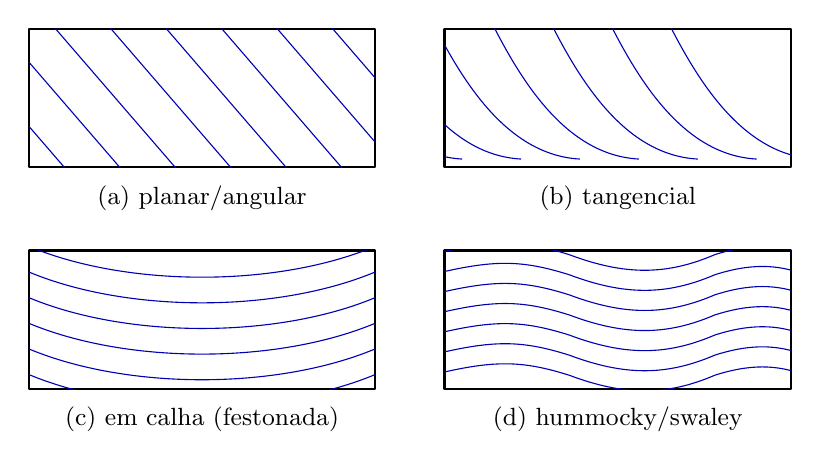
\begin{tikzpicture}[line cap=round,line join=round,scale=0.88,
                    every node/.style={font=\small}]
  % (a) Planar/angular: limites planos e lâminas inclinadas retas.
  \begin{scope}[shift={(0,3.2)}]
    \draw[thick] (0,0) rectangle (5,2);
    \begin{scope}
      \clip (0,0) rectangle (5,2);
      \foreach \x in {-1.3,-0.5,0.3,1.1,1.9,2.7,3.5,4.3} {
        \draw[blue!70!black] (\x,2.1)--({\x+1.9},-0.1);
      }
    \end{scope}
    \node[below] at (2.5,-0.12) {(a) planar/angular};
  \end{scope}
  % (b) Tangencial: lâminas se achatam ao aproximar-se da base.
  \begin{scope}[shift={(6,3.2)}]
    \draw[thick] (0,0) rectangle (5,2);
    \begin{scope}
      \clip (0,0) rectangle (5,2);
      \foreach \x in {-1.9,-1.05,-0.2,0.65,1.5,2.35,3.2} {
        \draw[blue!70!black] (\x,2.15)
          .. controls ({\x+0.45},1.25) and ({\x+1.1},0.18) ..
          ({\x+2.15},0.12);
      }
    \end{scope}
    \node[below] at (2.5,-0.12) {(b) tangencial};
  \end{scope}
  % (c) Calha: cortes côncavos sucessivos.
  \begin{scope}[shift={(0,0)}]
    \draw[thick] (0,0) rectangle (5,2);
    \begin{scope}
      \clip (0,0) rectangle (5,2);
      \foreach \h in {0.35,0.72,1.09,1.46,1.83,2.20} {
        \draw[blue!70!black] (-0.3,\h)
          .. controls (1.2,{\h-0.78}) and (3.8,{\h-0.78}) ..
          (5.3,\h);
      }
    \end{scope}
    \node[below] at (2.5,-0.12) {(c) em calha (festonada)};
  \end{scope}
  % (d) Hummocky/swaley: laminações onduladas de baixo ângulo.
  \begin{scope}[shift={(6,0)}]
    \draw[thick] (0,0) rectangle (5,2);
    \begin{scope}
      \clip (0,0) rectangle (5,2);
      \foreach \h in {0.20,0.49,0.78,1.07,1.36,1.65,1.94} {
        \draw[blue!70!black] (-0.2,\h)
          .. controls (0.7,{\h+0.22}) and (1.1,{\h+0.22}) ..
          (1.8,\h)
          .. controls (2.6,{\h-0.30}) and (3.2,{\h-0.30}) ..
          (3.9,\h)
          .. controls (4.4,{\h+0.16}) and (4.8,{\h+0.16}) ..
          (5.2,\h);
      }
    \end{scope}
    \node[below] at (2.5,-0.12) {(d) hummocky/swaley};
  \end{scope}
\end{tikzpicture}
\caption{Comparação esquemática de geometrias internas de estratificação.
Os retângulos representam os limites externos de cada intervalo; as linhas
azuis representam lâminas preservadas. O quadro (d) representa estruturas
de ondas e fluxos combinados, não a migração simples de uma duna.
Desenhos sem escala.}
\label{fig:tipos-estratificacao}
\end{figure}

\subsection{Seixos imbricados}

\emph{Imbricação} é o arranjo preferencial de clastos, sobretudo seixos
achatados, que se sobrepõem como telhas. Em muitos depósitos de corrente,
seus planos mergulham para montante. A orientação de vários seixos pode
indicar a paleocorrente, mas uma pedra isolada não é suficiente; deve-se
verificar também se a camada não foi inclinada posteriormente.

\begin{figure}[htbp]
\centering
\begin{tikzpicture}[>=Stealth,scale=0.83]
  \draw[->,thick] (3.3,1.5)--(5.4,1.5) node[right]{fluxo};
  \draw[thick] (0,0)--(6.3,0);
  \foreach \x in {0.8,1.7,2.6,3.5,4.4,5.3} {
    \draw[thick,rotate around={25:(\x,0.52)}]
      (\x,0.52) ellipse (0.62 and 0.19);
  }
  \node[below] at (1,-0.1) {montante};
  \node[below] at (5.1,-0.1) {jusante};
\end{tikzpicture}
\caption{Seixos imbricados com planos mergulhando para montante.
Esquema sem escala.}
\label{fig:seixos-imbricados}
\end{figure}

\subsection{Forma dos grãos e feições superficiais}

A forma de um grão inclui sua esfericidade, seu arredondamento e, no caso
de clastos maiores, a proporção entre seus eixos. Suas feições superficiais
podem registrar episódios sucessivos de transporte, alteração e deformação.
Nenhuma marca isolada prova um ambiente de formação.

\begin{description}[leftmargin=2.7cm,style=nextline]
  \item[Facetas] Superfícies relativamente planas produzidas por desgaste,
  fratura ou contato com outros materiais. Devem ser interpretadas junto
  com outras feições e com o contexto do depósito.
  \item[Cavidades] Depressões ou marcas superficiais que podem decorrer de
  impactos, dissolução ou alteração. É preciso registrar tamanho, forma e
  distribuição antes de atribuir-lhes uma origem.
  \item[Achatamento] Forma em que uma dimensão do clasto é menor que as
  demais. Pode ser herdada da rocha fonte, resultar de desgaste seletivo ou
  de deformação posterior. Favorece a formação de arranjos imbricados.
  \item[Estrias] Riscos e sulcos estreitos produzidos por abrasão ou atrito.
  Podem ocorrer em clastos transportados por geleiras, mas uma interpretação
  glacial requer outras evidências associadas
  \autocite{trosdtorf2005glacial}.
\end{description}

\subsection{Camadas maciças e deformação de sedimentos moles}

Uma camada \emph{maciça} não apresenta laminação interna facilmente
reconhecível na escala observada. Trata-se de uma descrição, não de um
processo único. A aparência pode resultar de sedimentação rápida de
material relativamente homogêneo, deposição por fluxos concentrados,
mistura biológica que apagou estruturas anteriores ou ausência de
contrastes visíveis entre lâminas \autocite{iodpestrutura,iodpbioturbacao}.

Fluxos de detritos ricos em sedimentos podem comportar-se como misturas
viscosas, transportando partículas de tamanhos diversos. Para interpretar
uma camada como produto desse processo, observam-se também seleção,
suporte dos clastos, contatos e associação com outras fácies. A aparência
maciça, sozinha, não é diagnóstica.

\paragraph{Escape de fluido.}
Sedimentos recém-depositados podem conservar muita água nos poros.
Sob carregamento rápido, a água escapa e pode deformar as laminações,
formar condutos ou produzir pequenos vulcões de areia. Essas feições
indicam mobilização após a deposição inicial e antes da completa
consolidação \autocite{kgsheterolitica}.

\paragraph{Dobramento sedimentar.}
Um escorregamento de sedimentos ainda pouco consolidados pode inclinar
e dobrar camadas; laminações convolutas também podem ocorrer em intervalos
restritos. Para distinguir esse dobramento de deformação tectônica
posterior, examinam-se os limites do intervalo deformado, as camadas
vizinhas e sua relação com o relevo deposicional
\autocite{kgsheterolitica}.

\subsection{Bioturbação, traços fósseis e icnofósseis}

\emph{Bioturbação} é a perturbação do sedimento pela atividade de
organismos, incluindo escavação, alimentação e deslocamento. Ela pode
preservar galerias reconhecíveis ou destruir quase toda a laminação,
deixando uma textura aparentemente homogênea \autocite{iodpbioturbacao}.

\emph{Traço fóssil} e \emph{icnofóssil} são nomes equivalentes para a
evidência preservada de atividade biológica, como pistas e galerias.
Bioturbação nomeia o processo e seu efeito sobre o sedimento; nem toda
camada bioturbada conserva um traço individual identificável
\autocite{kuichnologia}.

\subsection{Gretas de ressecamento e argilominerais}

\emph{Gretas de ressecamento} se abrem quando um sedimento úmido perde
água e se contrai. Em planta, podem delimitar polígonos; em corte,
frequentemente se estreitam para baixo. O preenchimento posterior
das fendas pode preservar seu molde nas rochas. Elas indicam exposição
e perda de água, embora seja necessário distinguir outras causas de
fraturamento por meio do contexto sedimentar.

Os argilominerais pertencem aos \emph{filossilicatos}, minerais de
estrutura em folhas. Alguns, especialmente os do grupo da esmectita,
incorporam água entre camadas e podem expandir-se ao hidratar e contrair
ao secar. Essa variação pode favorecer o desenvolvimento de gretas.
Nem todos os argilominerais são igualmente expansivos; a greta, sozinha,
não identifica sua composição \autocite{usgsargilas}.

\subsection{Estruturas heterolíticas}

Depósitos \emph{heterolíticos} alternam areia e lama. Correntes mais
ativas podem transportar areia junto ao fundo, ao passo que a lama se
acumula durante intervalos de menor energia. Essa alternância ocorre
frequentemente em ambientes influenciados por marés, mas não é exclusiva
deles \autocite{kgsheterolitica}.

\begin{description}[leftmargin=3.1cm,style=nextline]
  \item[Acamamento flaser] Predomina a areia; finas porções descontínuas
  de lama podem ocupar as depressões de ripples arenosos.
  \item[Acamamento ondulado] Areia e lama formam lâminas onduladas mais
  contínuas, com presença relativamente equilibrada dos dois materiais.
  \item[Acamamento lenticular] Predomina a lama, com lentes de areia
  isoladas ou pouco conectadas.
\end{description}

Para sustentar uma interpretação de marés, convém procurar também
reversão de paleocorrentes, superfícies de reativação e outras evidências
na associação de fácies \autocite{kgsheterolitica}.

\subsection{Marcas de sola, turboglifos e marcas de objeto}

\emph{Marcas de sola} são feições preservadas na superfície inferior de
uma camada. Muitas começam como depressões escavadas em lama; a areia
depositada depois as preenche e conserva um contramolde em relevo na
base do arenito \autocite{solemarks1957}.

\paragraph{Turboglifos.}
Os turboglifos (\emph{flute marks}) são escavações alongadas e assimétricas
produzidas pelo fluxo sobre um fundo coeso. Seus contramoldes são os
\emph{flute casts}. No caso típico, a extremidade mais larga e abrupta
aponta para montante e a parte afilada se prolonga para jusante,
indicando o sentido da paleocorrente \autocite{solemarks1957,kgssolemarks}.

\paragraph{Marcas de objeto.}
Seixos, conchas e fragmentos transportados podem tocar, arrastar-se ou
ricochetear no fundo, produzindo sulcos e marcas de impacto
(\emph{tool marks}). Sulcos longos frequentemente indicam a orientação
do movimento, mas nem sempre seu sentido. Turboglifos e marcas de objeto
são tipos distintos de marcas que podem ser preservadas na sola de uma
camada \autocite{solemarks1957}.

% ----------------------------------------------------------------------
% REFERÊNCIAS NOVAS: copie as entradas abaixo, SEM o sinal % inicial,
% para o arquivo referencias.bib que já acompanha seu documento.
% A entrada trosdtorf2005glacial foi fornecida anteriormente.
%
% @online{southard2006bedforms,
%   author = {Southard, John},
%   title = {Bed Configurations Generated by Water Flows and Wind},
%   organization = {MIT OpenCourseWare}, year = {2006},
%   url = {https://ocw.mit.edu/courses/12-090-introduction-to-fluid-motions-sediment-transport-and-current-generated-sedimentary-structures-fall-2006/resources/ch12/},
%   urldate = {2026-09-28}}
% @online{southard2006cross,
%   author = {Southard, John}, title = {Cross Stratification},
%   organization = {MIT OpenCourseWare}, year = {2006},
%   url = {https://ocw.mit.edu/courses/12-090-introduction-to-fluid-motions-sediment-transport-and-current-generated-sedimentary-structures-fall-2006/resources/ch16/},
%   urldate = {2026-09-28}}
% @online{iodpestrutura,
%   author = {{International Ocean Discovery Program}},
%   title = {Sediment Description: Sedimentary Structures},
%   url = {https://iodp.tamu.edu/publications/TN/Appendix/Appendix_4.1.pdf},
%   urldate = {2026-09-28}}
% @online{iodpbioturbacao,
%   author = {{Ocean Drilling Program}}, title = {Methods: Sediment Description},
%   url = {https://www.iodp.tamu.edu/publications/exp302/103/103_2.htm},
%   urldate = {2026-09-28}}
% @online{kgsheterolitica,
%   author = {{Kansas Geological Survey}},
%   title = {Sedimentology and Ichnology of Paleozoic Estuarine and Shoreface Reservoirs},
%   url = {https://www.kgs.ku.edu/Current/1999/buatois/buatois5.html},
%   urldate = {2026-09-28}}
% @online{kuichnologia,
%   author = {{University of Kansas}}, title = {Glossary: Ichnology},
%   url = {https://ichnology.ku.edu/poi/poi/glossary.html},
%   urldate = {2026-09-28}}
% @online{usgsargilas,
%   author = {{U.S. Geological Survey}},
%   title = {Environmental Characteristics of Clays and Clay Mineral Deposits},
%   url = {https://pubs.usgs.gov/info/clays/},
%   urldate = {2026-09-28}}
% @article{solemarks1957,
%   title = {Sole Markings of Graded Graywacke Beds},
%   journaltitle = {The Journal of Geology}, year = {1957},
%   volume = {65}, number = {3}, doi = {10.1086/626429}}
% @online{kgssolemarks,
%   author = {{Kansas Geological Survey}},
%   title = {Ichnology of a Pennsylvanian Equatorial Tidal Flat: Sedimentology},
%   url = {https://www.kgs.ku.edu/Publications/Bulletins/245/03_sedim.html},
%   urldate = {2026-09-28}}
% @online{usgshummocky,
%   author = {{U.S. Geological Survey}},
%   title = {Cyclic Deposits and Hummocky Cross-Stratification of Probable
%            Storm Origins in Upper Cretaceous Rocks of the Cape Sebastian Area},
%   url = {https://pubs.usgs.gov/publication/70011848},
%   urldate = {2026-09-29}}
